\section{Results}
\label{sec:results}

\begin{figure} 	
\centering 	
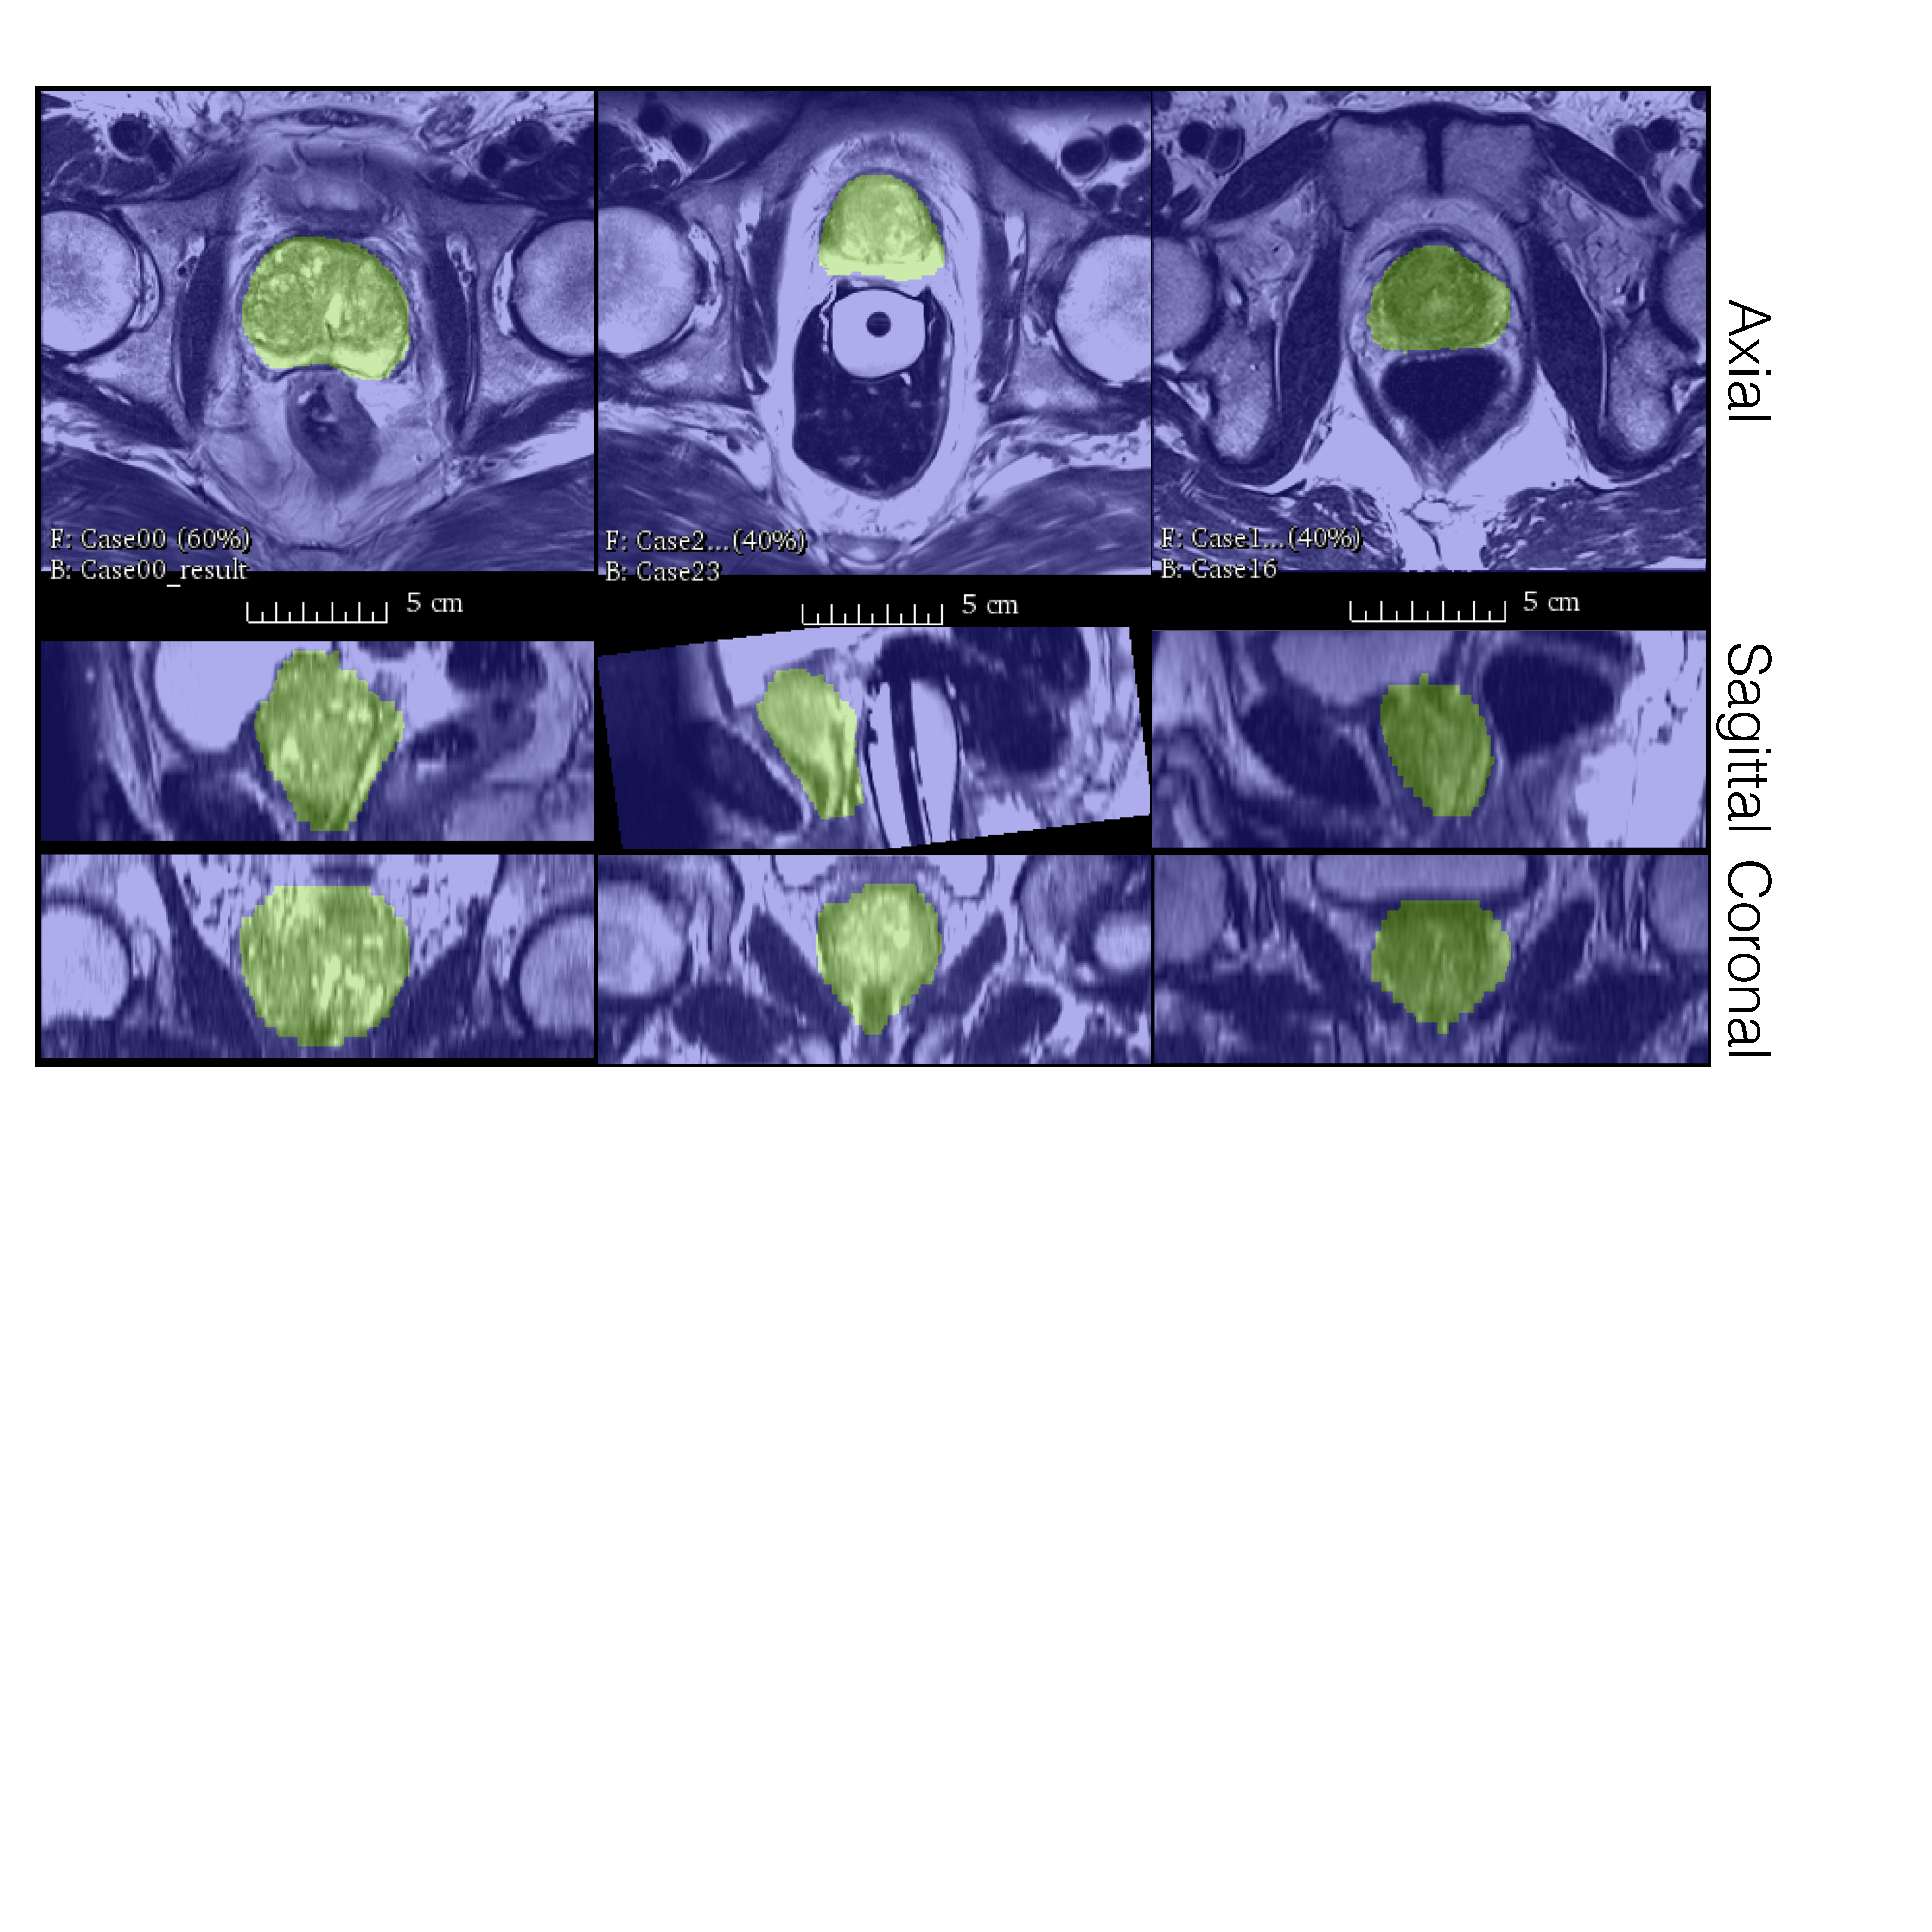
\includegraphics[scale=0.18]{qualitativeResults.pdf} 	
\caption{Qualitative results on the PROMISE 2012 dataset \cite{litjens2014evaluation}.} \label{fig:qualitative} 
\end{figure}

We trained our method on $50$ MRI volumes, and the relative manual ground truth annotation, obtained from the "PROMISE2012" challenge dataset \cite{litjens2014evaluation}. This dataset contains medical data acquired in different hospitals, using different equipment and different acquisition protocols. The data in this dataset is representative of the clinical variability and challenges encountered in clinical settings. As previously stated we massively augmented this dataset through random transformation performed in each training iteration, for each mini-batch fed to the network. The mini-batches used in our implementation contained two volumes each, mainly due to the high memory requirement of the model during training. We used a momentum of $0.99$ and a initial learning rate of $0.0001$ which decreases by one order of magnitude every $25$K iterations. 

\begin{figure} 	
\centering 	
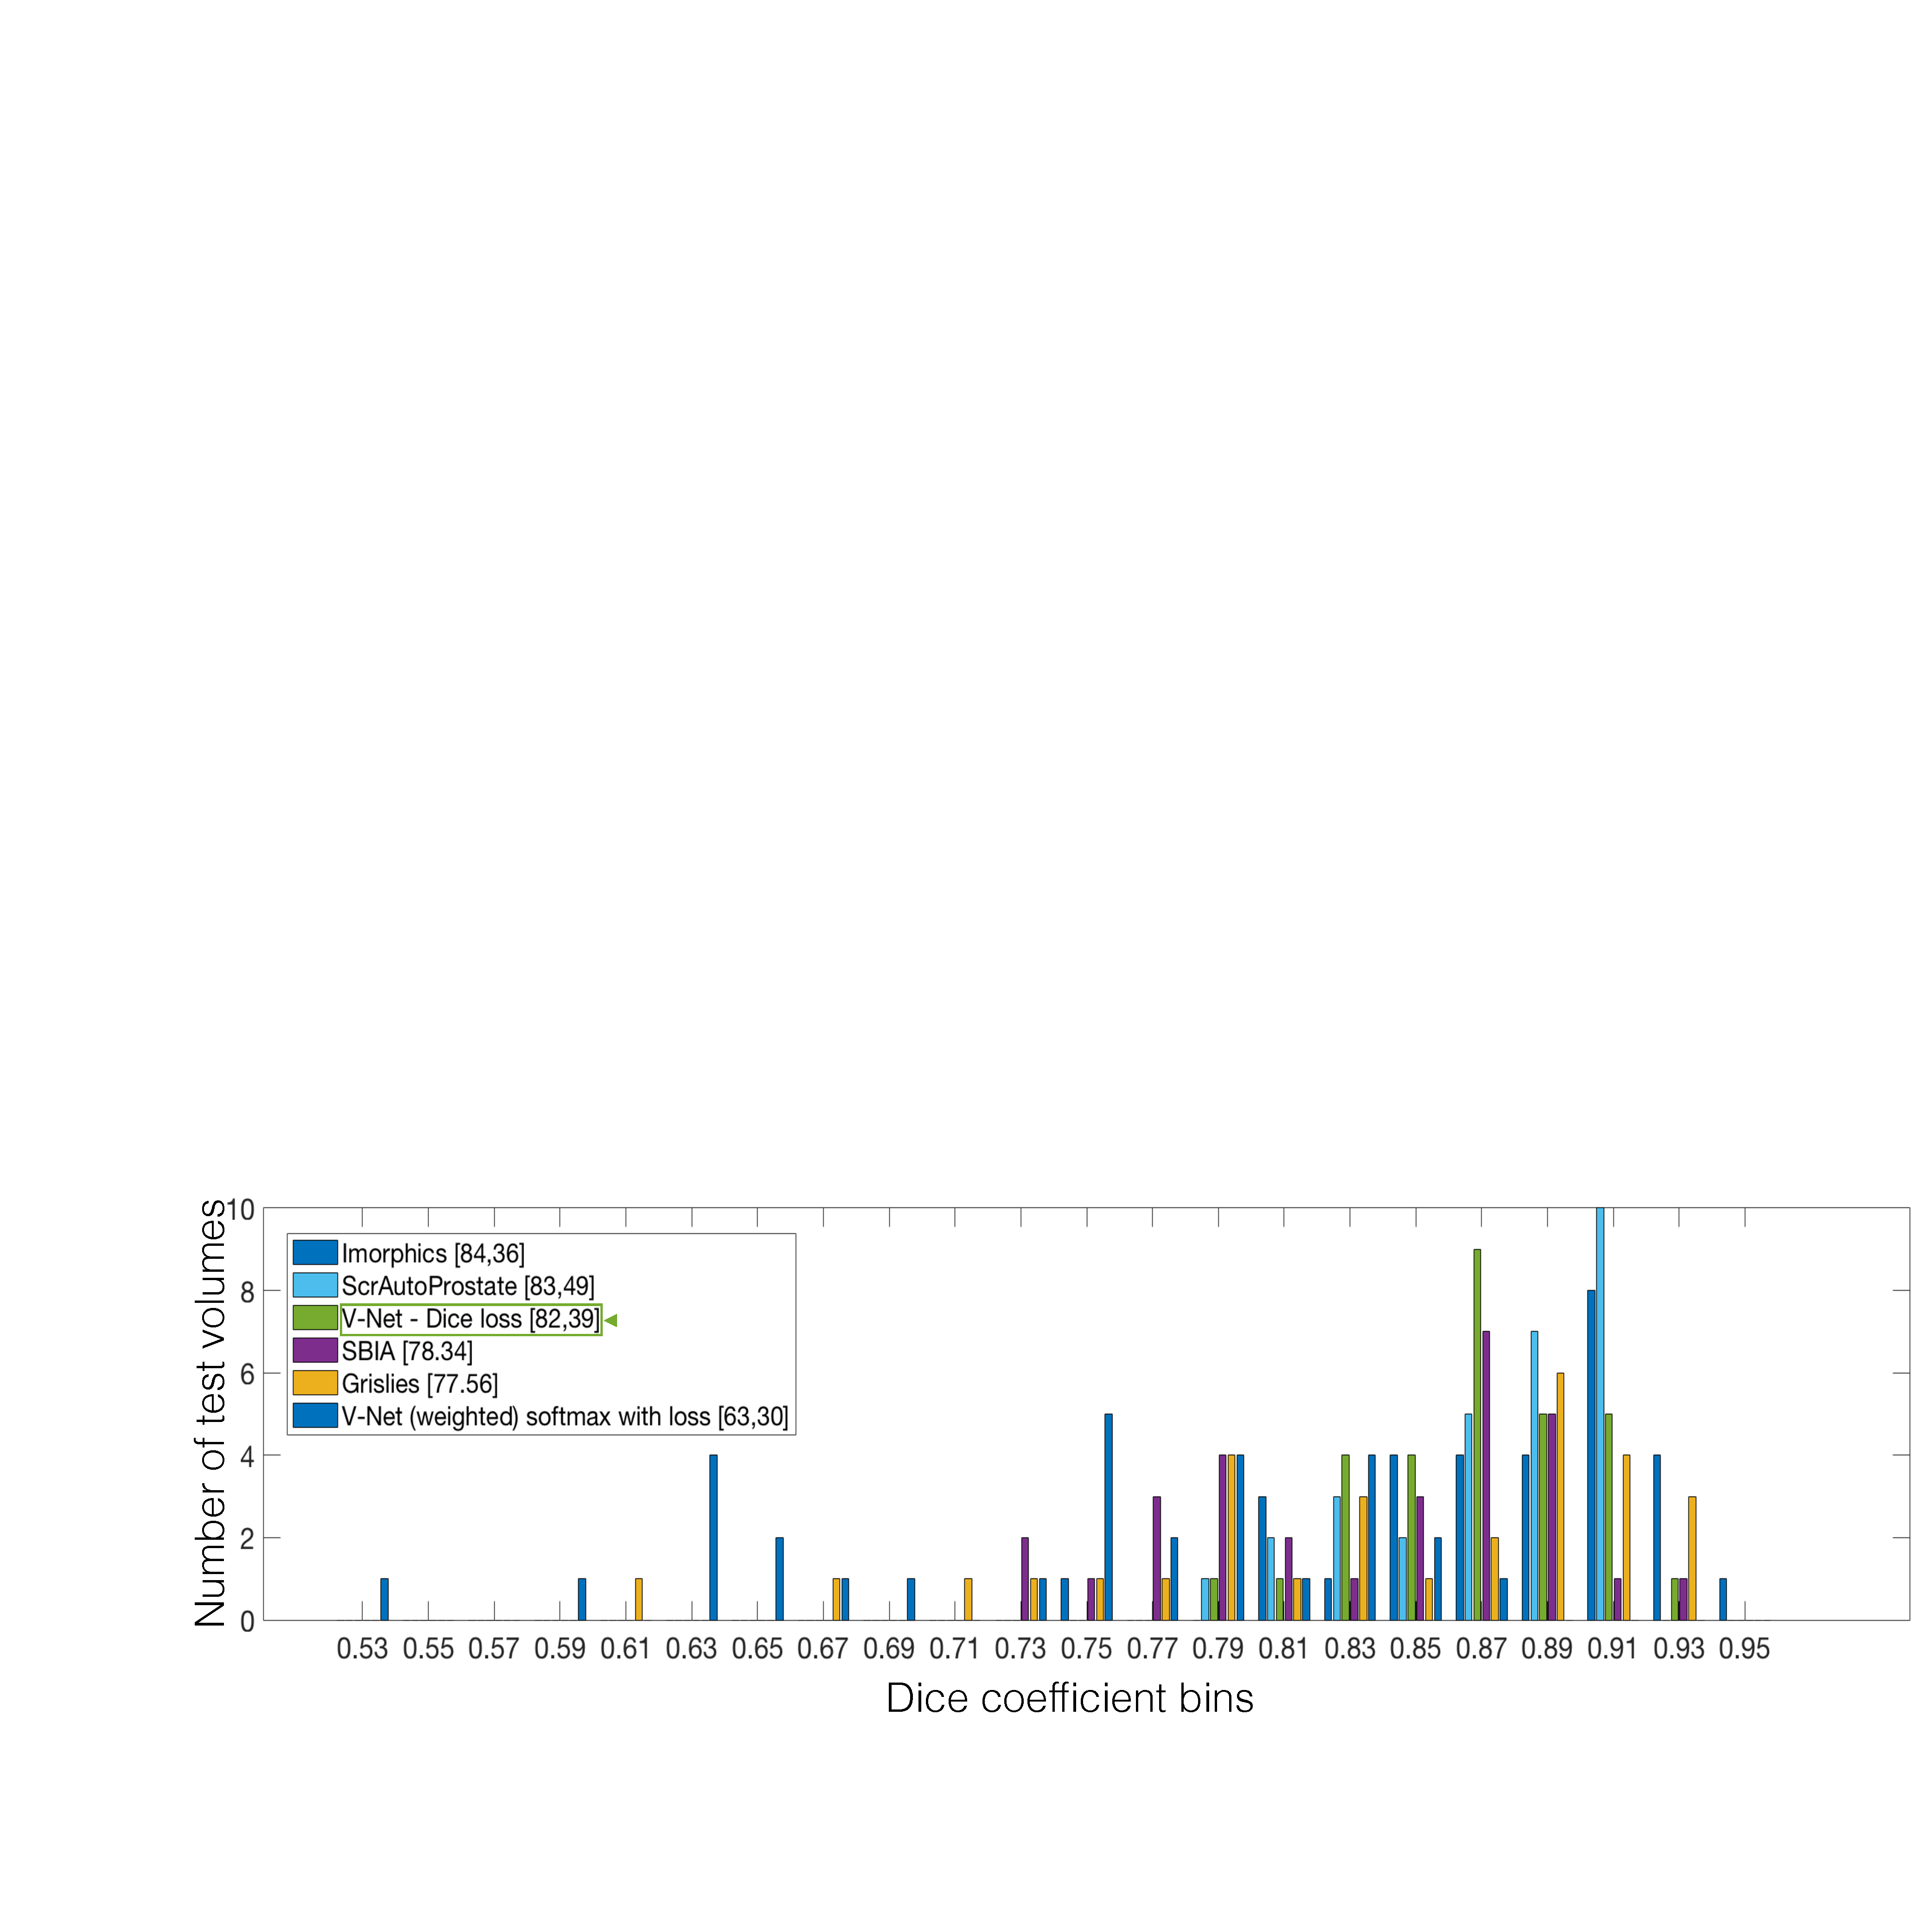
\includegraphics[scale=0.19]{histogram.pdf} 	
\caption{Distribution of volumes with respect to the Dice coefficient achieved during segmentation.} 
\label{fig:hist} 
\end{figure}

We tested V-Net on $30$ MRI volumes depicting prostate whose ground truth annotation was secret. All the results reported in this section of the paper were obtained directly from the organisers of the challenge after submitting the segmentation obtained through our approach. The test set was representative of the clinical variability encountered in prostate scans in real clinical settings \cite{litjens2014evaluation}. 

We evaluated the approach performance in terms of Dice coefficient, Hausdorff distance of the predicted delineation to the ground truth annotation and in terms of score obtained on the challenge data as computed by the organisers of "PROMISE 2012" \cite{litjens2014evaluation}. The results are shown in Table \ref{tab:res} and Fig. \ref{fig:hist}.

\begin{table}
\caption{Quantitative comparison between the proposed approach and the current best results on the PROMISE 2012 challenge dataset.} \label{tab:res}
\begin{tabular}{|c|c|c|c|}
\hline 
Algorithm & Avg. Dice & Avg. Hausdorff distance & Score on challenge task\tabularnewline
\hline 
\hline 
V-Net + Dice-based loss & $0.869 \pm 0.033$ & $5.71 \pm 1.20$ mm & $82.39$\tabularnewline
\hline 
V-Net + mult. logistic loss & $0.739 \pm 0.088 $ & $10.55 \pm 5.38$ mm & $63.30$\tabularnewline
\hline 
Imorphics \cite{imorp} & $0.879 \pm 0.044$ & $5.935 \pm 2.14 $ mm & $84.36$\tabularnewline
\hline 
ScrAutoProstate & $0.874 \pm 0.036$ & $5.58 \pm 1.49 $ mm & $83.49$ \tabularnewline
\hline
SBIA & $0.835 \pm 0.055$ & $7.73 \pm 2.68 $ mm & $78.33$ \tabularnewline
\hline
Grislies & $0.834 \pm 0.082$ & $7.90 \pm 3.82 $ mm & $77.55$ \tabularnewline
\hline

\end{tabular}

\end{table}

\begin{figure} 	
\centering 	
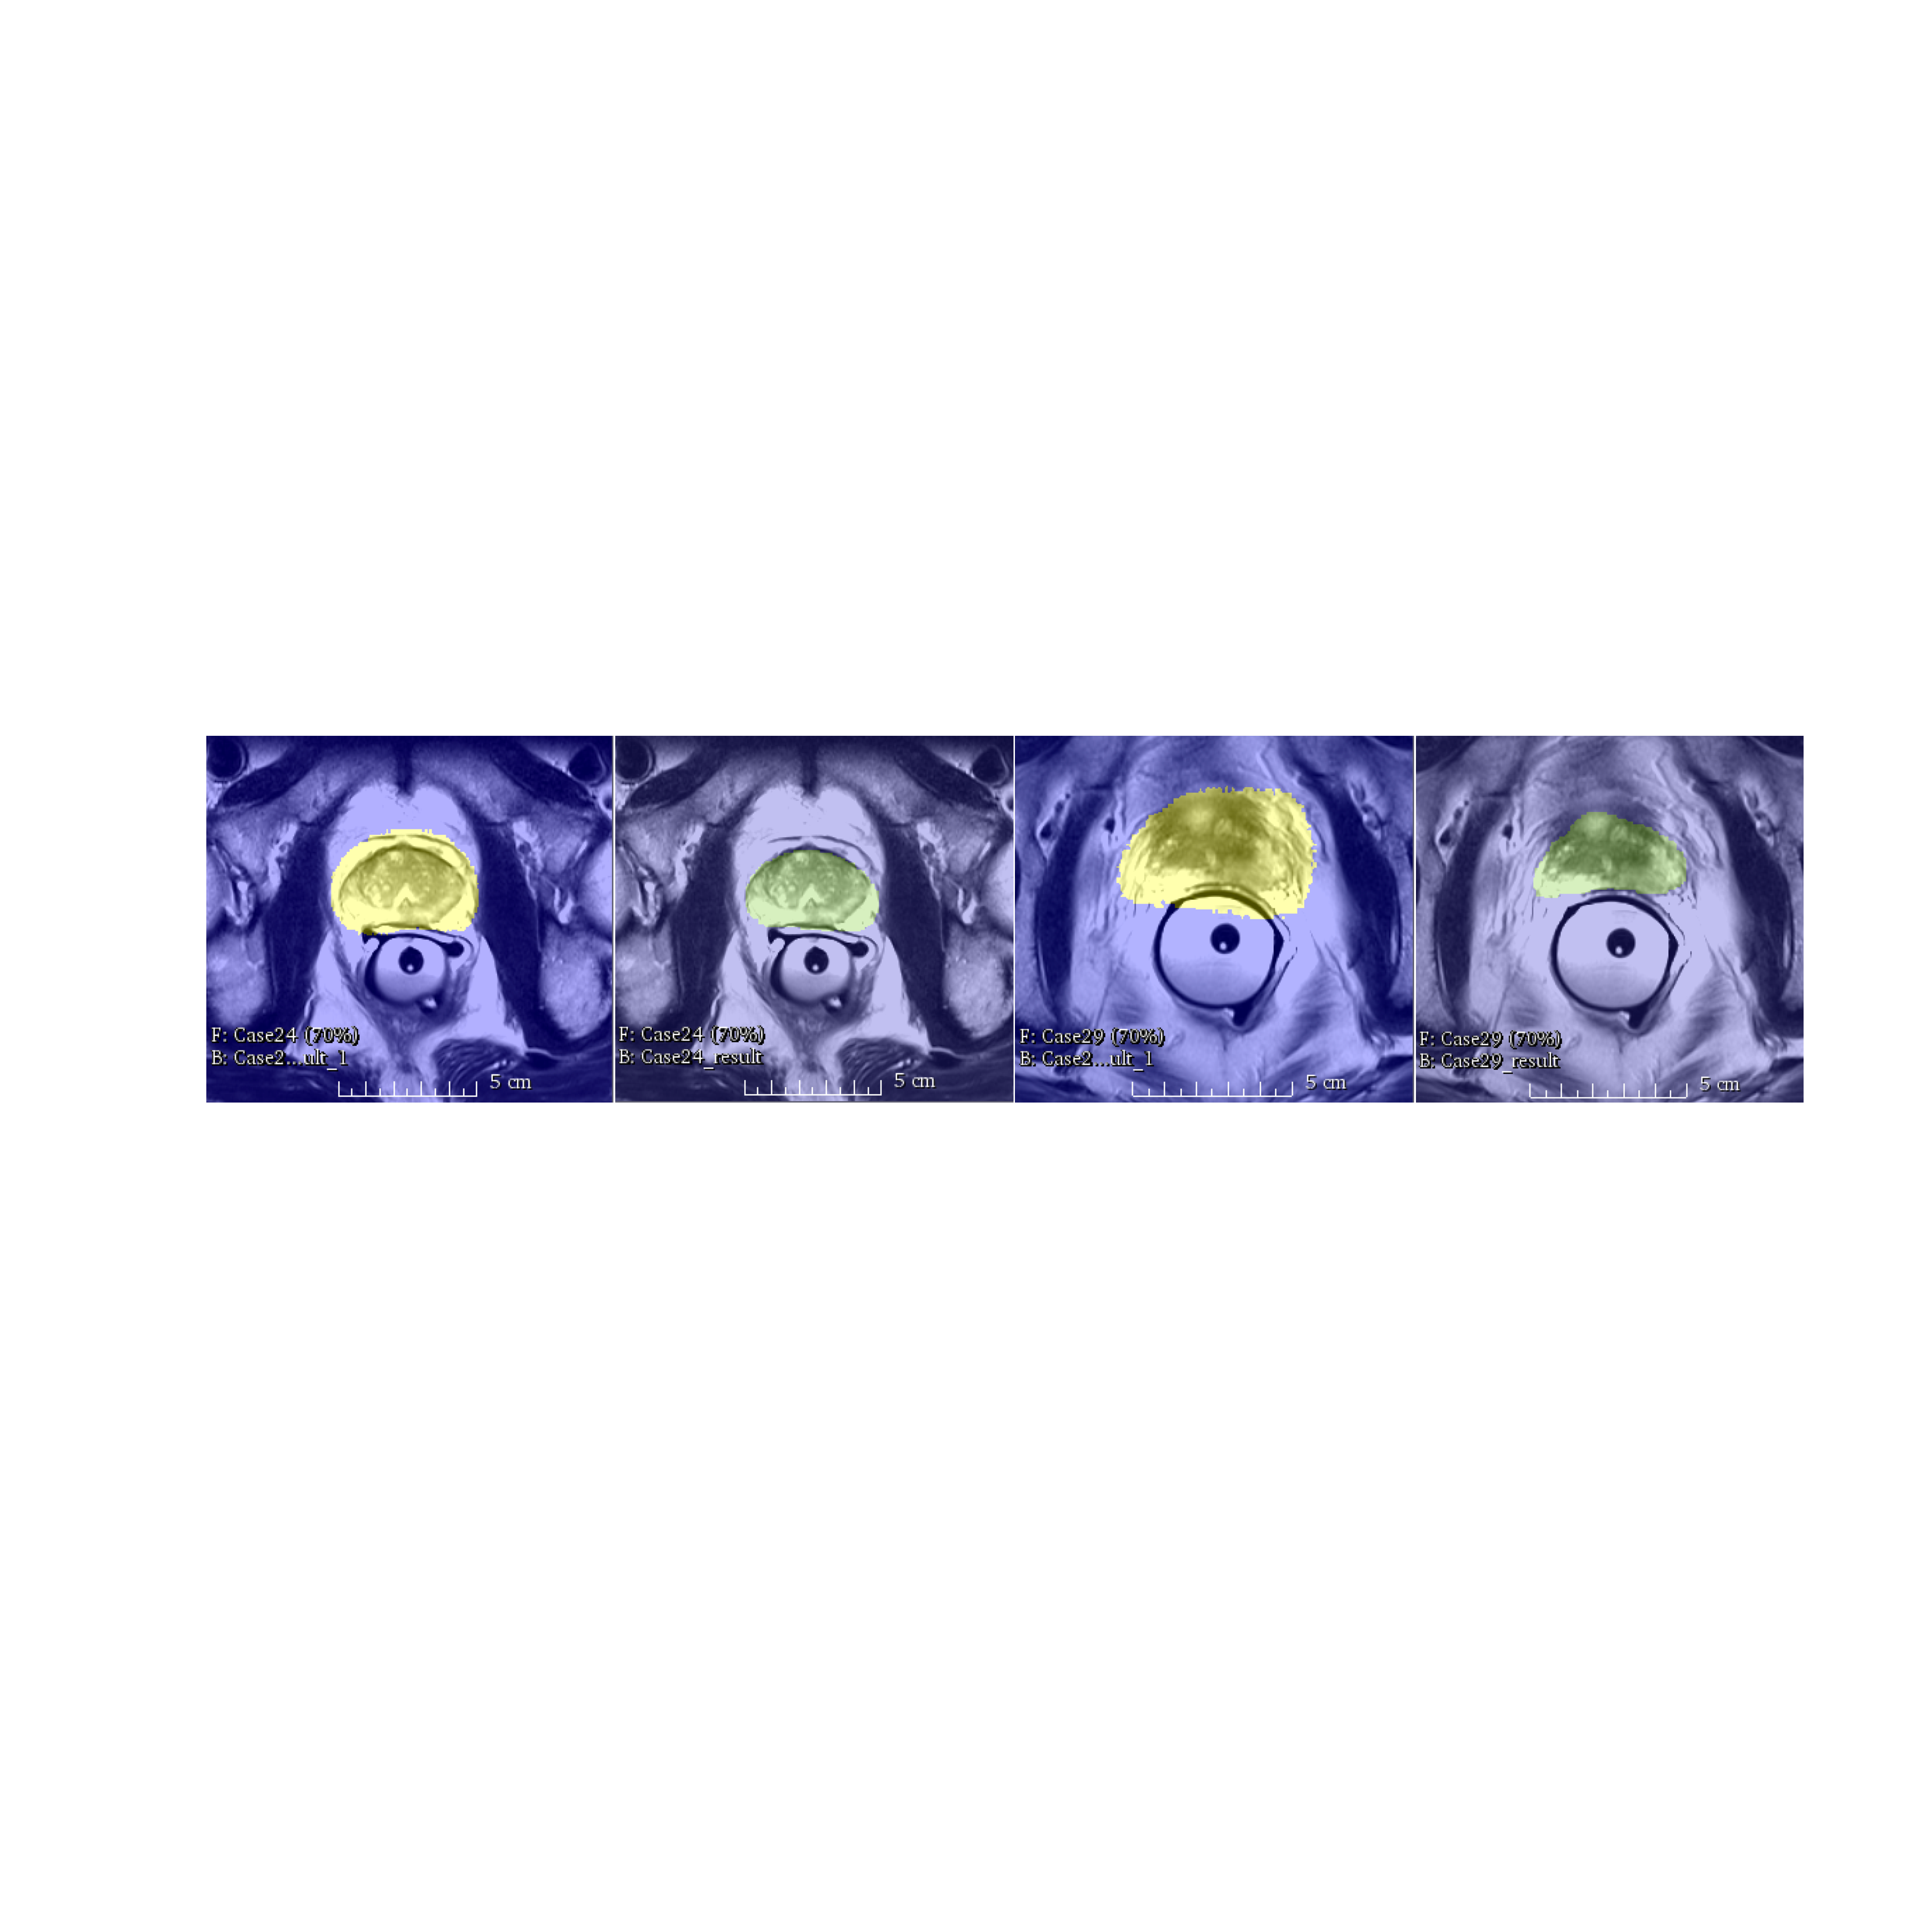
\includegraphics[scale=0.208]{dice_vs_softmaxwithloss.pdf} 	
\caption{Qualitative comparison between the results obtained using the Dice coefficient based loss (green) and re-weighted soft-max with loss (yellow).} \label{fig:qualitativecomparison} 
\end{figure}

Our implementation\footnote{Implementation available at \url{https://github.com/faustomilletari/VNet}} was realised in python, using a custom version of the Caffe\footnote{Implementation available at \url{https://github.com/faustomilletari/3D-Caffe}} \cite{jia2014caffe} framework which was enabled to perform volumetric convolutions via CuDNN v3. All the trainings and experiments were ran on a standard workstation equipped with $64$ GB of memory, an Intel(R) Core(TM) i7-5820K CPU working at 3.30GHz, and a NVidia GTX 1080 with $8$ GB of video memory. We let our model train for $48$ hours, or $30$K iterations circa, and we were able to segment a previously unseen volume in circa $1$ second. The datasets were first normalised using the N4 bias filed correction function of the ANTs framework \cite{tustison2010n4itk} and then resampled to a common resolution of $1\times1\times1.5$ mm. We applied random deformations to the scans used for training by varying the position of the control points with random quantities obtained from gaussian distribution with zero mean and $15$ voxels standard deviation. Qualitative results can be seen in Fig. \ref{fig:qualitative}.